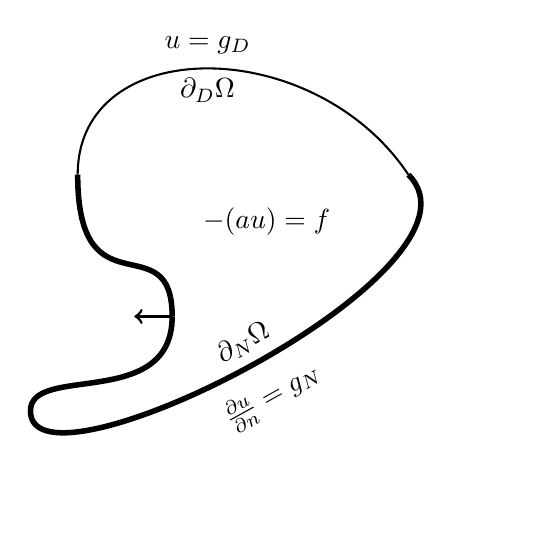
\begin{tikzpicture}[scale=0.6]
\draw[line width=0.75pt] (0,0) .. controls (0,3) and (5,3) .. node[sloped,above,yshift=0.5mm] {$u=g_D$} node[sloped,below] {$\partial_D\Omega$} (7,0);
\draw[line width=2pt] (7,0) .. controls (9,-2) and (-1,-7) .. node[sloped,above] {$\partial_N\Omega$} node[sloped,below,yshift=-1mm] {$\frac{\partial u}{\partial n} = g_N$} (-1,-5);
\draw[line width=2pt] (-1,-5) .. controls (-1,-4) and (2,-5) .. (2,-3);
\draw[line width=2pt] (2,-3) .. controls (2,-1) and (0,-3) .. (0,0);
\draw[->,line width=1.0pt] (2,-3) -- (1.2,-3) node[below] {$\bn$}; % normal vector
\draw (4,-1) node {$- \Div (a \grad u) = f$};
\end{tikzpicture}

